% ---------------------------------------------------------------------------
% External validation. Numbers from validate_cimmyt.py; see
% results/V1_cimmyt_summary.json.
% ---------------------------------------------------------------------------

\section{External Validation}
\label{sec:validation}

A simulation study is only as good as the biology inside it, so we test the
model against a dataset that played no part in building it.
Chassaigne-Ricciulli \textit{et al.}~\cite{chassaigne2021} report seed
production technology for six three-way-cross tropical maize hybrids at
CIMMYT's station in Agua Fr\'ia, Mexico, giving for each hybrid the parents'
accumulated growing degree days at flowering, the differential sowing
interval they recommend, and a ranking of the six by difficulty of seed
production. None of it entered our model: the yield response comes from
Nepal~\cite{marahatta2025} and the phenology from DSSAT's genotype
database~\cite{dssat}.

\textit{Parameters corroborated.} Both studies compute thermal time
identically --- daily mean above a $10^\circ$C base, truncated at
$30^\circ$C --- so the thermal model underlying the scheduler is the one the
field uses. CIMMYT estimate ``7 days for the total pollen shedding
duration,'' which is the value our floral-overlap term assumes, and report
stigmas receptive about five days after the onset of female flowering,
inside our six-day stand-level window. The one component of the yield
response that we extended beyond the fitted data is therefore supported by
measurements from another continent.

\textit{Recommended offsets reproduced.} The model's core biological claim is
that the sowing offset needed to synchronise two parents equals their
thermal-time difference divided by the rate at which degree days accumulate,
and CIMMYT publish both sides of that equation. Using their reported parent
GDD values and measured accumulation rate, the model predicts their
recommended offsets with a mean absolute error of 1.5~days and recovers the
correct direction --- which parent is sown first --- in six cases of six
(Fig.~\ref{fig:cimmyt}(a)). For the three hybrids reporting both parents'
GDD separately, predicted and recommended offsets correlate at $r = 0.99$,
illustrative rather than conclusive at $n = 3$.

\textit{Difficulty ranking reproduced.} Ranking the same six hybrids by the
offset our model requires reproduces CIMMYT's own ordering at Spearman
$\rho = 0.71$ (Fig.~\ref{fig:cimmyt}(b)) --- suggestive rather than
significant with six hybrids, and reported as such.

This establishes that the biology driving the scheduler behaves like the
published biology, and that the hybrids our model finds hard to schedule are
the ones practitioners find hard to produce. It does not validate the
scheduler: no one has executed one of our schedules on real fields and
weighed the resulting seed, and nothing short of that would. What it buys is
the right to read differences between strategies as differences in scheduling
quality rather than artefacts of a misspecified crop response.

\begin{figure}[t]
\centering
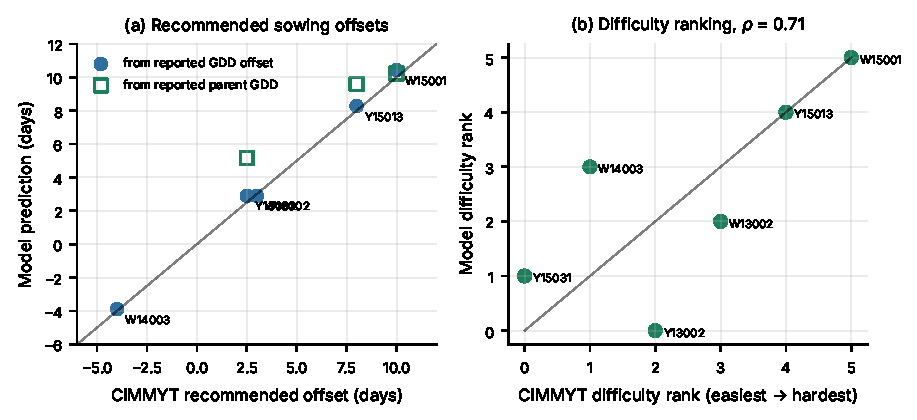
\includegraphics[width=\columnwidth]{../figs/fig7_cimmyt.pdf}
\caption{External validation against CIMMYT's published seed-production
recommendations~\cite{chassaigne2021}. (a) Predicted against recommended
sowing offsets for six three-way-cross hybrids; the line is parity.
(b) Hybrid difficulty ranking.}
\label{fig:cimmyt}
\end{figure}

\textit{The assumption this study removes.} Recommending that males be sown
on two consecutive dates, the same paper states that ``it is assumed that
machinery is available to do the sowing, or, in the case of rains after the
first sowing, staff are available to planting,'' and elsewhere describes a
second male date sown ``anticipating a lag with the first date due to some
unforeseen rain.'' That assumption is this paper's subject. The agronomic
literature derives the offsets each hybrid needs and supposes the crew will
be free to deliver them; we ask what happens when one crew serves many fields
and rain closes some of them. We also adopt their two-date male sowing, which
raises the work per field from two crew visits to three.
